\chapter{Glavne komponente}

V prejšnjih dveh poglavjih smo spoznavali neposredne koristi pristopa k analizi podatkov, kjer za dani model in kriterijsko funkcijo uporabimo strojno odvajanje in gradientni sestop in potem uživamo v rezultatih. Model je bil v prejšnjih dveh poglavjih isti in silno enostaven. Linearna regresija ima prednost, da je model berljiv in podan z utežmi, z uporabo enostavnega trika, regularizacije, pa ga lahko še dodatno zgladimo (regularizacija L2) ali pa poenostavimo (regularizacija L1).

Lahko podoben pristop uporabimo za nek popolnoma drugačen model? Tu ne mislimo na napovedne modele, ampak, na primer, na model projekcije ali pa vložitve podatkov. Lahko, ampak da ne prehitevamo: v tem in naslednjem poglavju bo govora o zmanjšanju dimenzij. Tu, v tem poglavju, z iskanjem projekcij, v naslednjem pa z vložitvami. A začnimo na začetku, s primerom in motivacijo.

\section{Razpršenost in varianca}

Prikazana sta dva primera dvodimenzionalnih podatkov. Pri obeh primerih smo podatke standardizirali. Pri prvem so podatki razpršeni po vsem podatkovnem prostoru, pri drugem imajo strukturo, saj sta atributa korelirana, njuna kovarianca je -0.9.

\begin{figure}
    \centering
    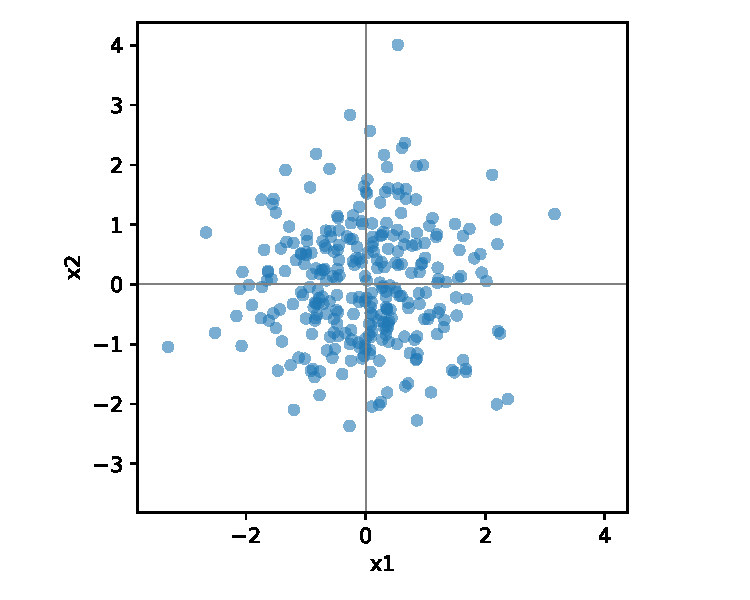
\includegraphics[width=0.48\linewidth]{figs/050-scatter-cor-zero.pdf}\hfill
    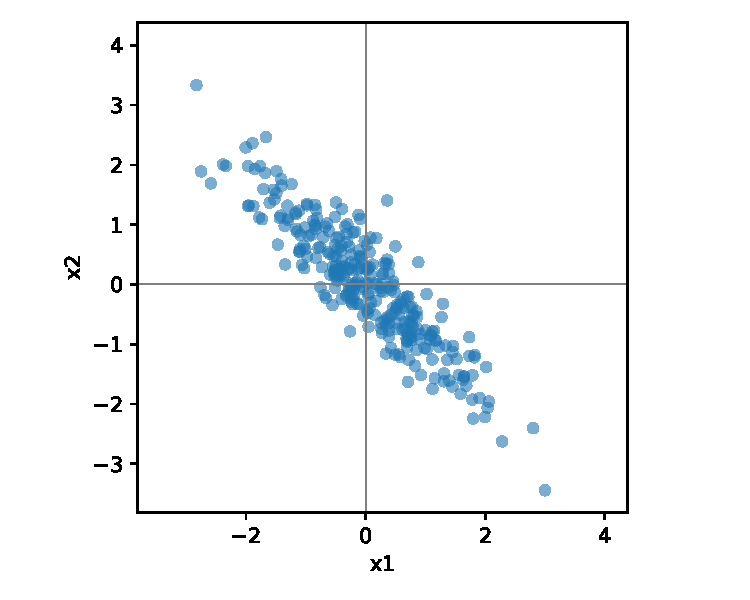
\includegraphics[width=0.48\linewidth]{figs/050-scatter-cor-high.pdf}
    \caption{Dva primera standardiziranih podatkov, prvi (levo) s kovarianco $0$ in drugi s kovarianco $-0,9$.}
    \label{fig:data}
\end{figure}

Pri generiranju dvodimenzionalnih normalno porazdeljenih podatkov z določeno kovarianco nam je pomagal \texttt{numpy}:
\vspace*{3mm}
\begin{lstlisting}
def generate_2d_normal(n, rho, rnd_seed=42):
    np.random.seed(rnd_seed)
    cov = np.array([[1.0, rho], [rho, 1.0]])
    data = np.random.multivariate_normal(mean=[0, 0], cov=cov, size=n)
    mean = data.mean(axis=0)
    std = data.std(axis=0)
    return (data - mean) / std
\end{lstlisting}

Želeli bi ugotoviti, v kateri smeri se podatki raztezajo, oziroma katera je smer, kjer so podatki najbolj razpršeni. Za naš primer s kovarianco $-0.9$ spodaj sta prikazani dve taki smeri, podani z dvema smernima vektorjema $a$ in $b$. 

\begin{figure}
    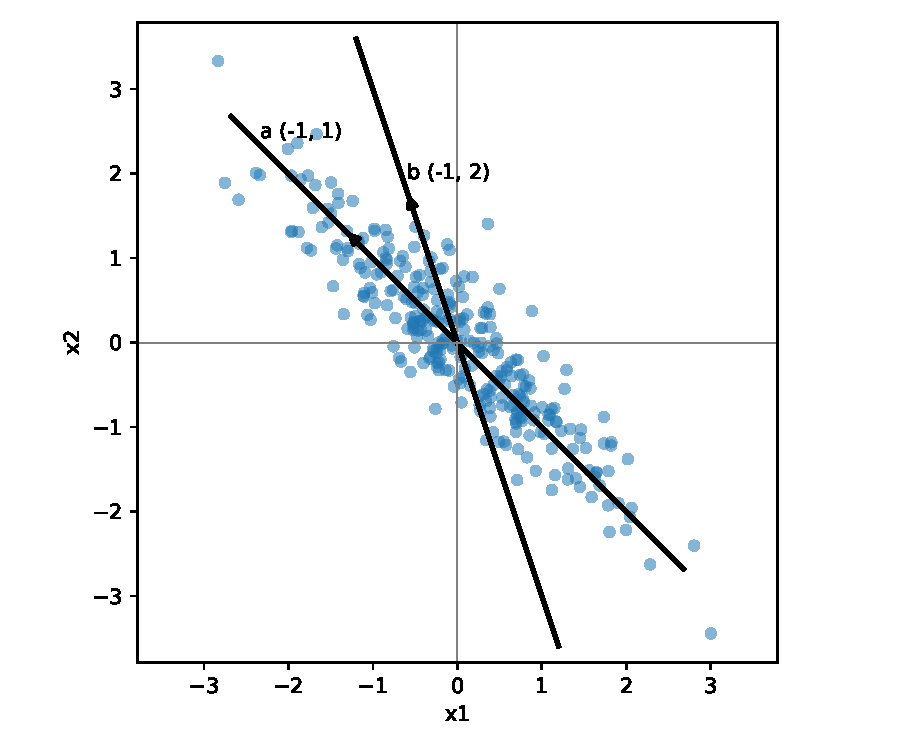
\includegraphics[width=0.5\textwidth]{figs/050-two-directions.pdf}
    \caption{Dve kandidatni smeri, po katerih lahko opazujemo razpršenost podatkov.}
    \label{fig:ab}
\end{figure}

Očitno so podatki bolj razpršeni v smeri vektorja $a$. A kako to pokažemo matematično? Razpršenost v statistiki merimo z varianco. Za enodimenzionalne podatke $z_1,\dots,z_n$ je varianca definirana kot
$$
\mathrm{Var}(z)=\frac{1}{n}\sum_{i=1}^n (z_i-\bar z)^2.
$$

Če želimo meriti razpršenost v določeni smeri, podatke projiciramo na enotni smerni vektor $u$, kjer velja $|u|=1$. Vektor $u$ izberemo kot smer v prostoru (npr. kandidatna smer $a$ ali $b$), ki jo želimo analizirati. Za smer $a$ bo smerni vektor $u=\frac{a}{|a|}$.

Naj bodo podatki zapisani v matriki $X\in\mathbb{R}^{n\times d}$, kjer vsaka vrstica predstavlja en primer. Ker so naši podatki dvodimenzionalni, ima matrika $X$ dve koloni. Projekcija podatkov na smer $u$ je potem podana kot
$$
X_u = X u,
$$
kjer $X_u\in\mathbb{R}^n$ predstavlja (enodimenzionalno) projekcijo naših podatkov. Smerni vektor\marginnote{Znova smo pri linearni kombinaciji atributov! Tudi tu ponovno srečamo uteži. Vodi to k interpretaciji rezultatov?} $u$ tudi določa uteži vhodnih atributov in torej njihovo linearno kombinacijo.

Za oba naša smerna vektorja lahko sedaj ugotovimo, kakšna je varianca, če podatke projiciramo na smeri, ki jih določata:
\vspace*{3mm}
\begin{lstlisting}
X = generate_2d_normal(n, rho=rho)
a = np.array([-1.0, 1.0])
b = np.array([-1.0, 3.0])
for v in [a, b]:
    var = projected_variance(X, v)
    print(f"Projected variance along ({v[0]}, {v[1]}): {var:.3f}")
\end{lstlisting}

Rezultat je pričakovan, podatki na projekciji na vektor $a$ so bolj razpršeni:
\vspace*{3mm}
\begin{lstlisting}
Projected variance along (-1.0, 1.0): 1.902
Projected variance along (-1.0, 3.0): 1.541
\end{lstlisting}

Lahko smerni vektor projekcije, kjer bi bili podatki najbolj razpršeni, poiščemo algoritmično? Lahko. Postopek se imenuje analiza glavnih komponent in jo bralec najbrž pozna, a bi jo tu (seveda) radi izvedli z gradientnim sestopom in z uporabo strojnega odvajanja.

\section{Iskanje glavne komponente}

Naj bo torej $u$ smer, na katero projiciramo podatke. Iščemo $u$, kjer so podatki najbolj razpršeni, torej kjer je varianca projekcije največja. Najprej zapišimo varianco projiciranih podatkov:
$$
\mathrm{Var}(X_u)=\frac{1}{n}\sum_{i=1}^n (x_i^\top u)^2,
$$
kjer smo upoštevali, da so podatki standardizirani in centrirani, zato je povprečje projekcije enako $0$. To lahko zapišemo v matrični obliki\marginnote{Pri tem zapisu smo si pomagali z dejstvom, da, če je $z$ skalar, velja $z=z\top$. Kako nam to pomaga?} kot
$$
\mathrm{Var}(X_u)=\frac{1}{n} u^\top X^\top X u.
$$

Določimo kriterijsko funkcijo
$$
J(u)=\frac{1}{n} u^\top X^\top X u,
$$
ki meri razpršenost podatkov v smeri $u$. Iščemo tak $u$, ki maksimizira $J(u)$, ob pogoju $|u|=1$. Tako dobimo optimizacijski problem
$$
\max_u J(u) \quad \text{pri pogoju} \quad |u|=1,
$$
ki ga lahko rešujemo z gradientnim sestopom (oziroma vzponom), pri čemer bomo morali po vsakem koraku vektor, ki osveži elemente vektorja $u$, ta vektor normirati, da zagotovimo, da ostane enoten.

Opisano funkcionalnost\marginnote{Malo nevšečno je, da moramo zato med parametre funkcije izgube vključiti \texttt{ys}, a spremembe funkcije \texttt{train}, ki bi omogočala klice brez \texttt{ys} in hkrati omogočala optimizacijo za linearno regresijo in iskanje glavne komponente prepuščamo bralcu.} implementirajmo v razredu \texttt{PCA1D}. Pri tem skušamo slediti strukturi implementacije linearne regresije, tako da ne spreminjamo ničesar v naši implementaciji gradientnega sestopa oziroma v funkciji \texttt{train}.

\vspace*{3mm}
\begin{lstlisting}
class PCA1D:
    def __init__(self, n_inputs, rnd_seed=42):
        rng = random.Random(rnd_seed)
        self.u = [Value(rng.uniform(-1, 1), label=f"u{i}") \
                  for i in range(n_inputs)]
        self.normalize_u()

    def parameters(self):
        return self.u

    def _dot(self, a, b):
        return sum(ai * bi for ai, bi in zip(a, b))

    def normalize_u(self, eps=1e-8):
        nrm = (self._dot(self.u, self.u) + eps) ** 0.5
        self.u = [ui / nrm for ui in self.u]

    def loss(self, xs, ys=None):
        self.normalize_u()
        total = Value(0.0, label="proj_var_sum")
        for x in xs:
            z = self._dot(x, self.u)
            total += z**2
        variance = total / len(xs)
        return -variance

    def batch_loss(self, xs, ys=None, m=20):
        indices = random.sample(range(len(xs)), m)
        batch_xs = [xs[idx] for idx in indices]
        return self.loss(batch_xs, ys=None)

    def explained_variance(self, xs):
        return -self.loss(xs, ys=None).data

    def __repr__(self):
        self.normalize_u()
        return "PCA1D(u=[" + \
               ", ".join(f"{ui.data:.3f}" for ui in self.u) + "])"
\end{lstlisting}

V kodi smo kriterijsko funkcijo obrnili v izgubo tako, da minimiziramo $-J(u)$ namesto da bi maksimizirali $J(u)$. To nam omogoča, da brez sprememb uporabimo isti postopek učenja kot prej. Ker mora biti $u$ enotni smerni vektor, ga v funkciji \texttt{normalize\_u} po vsakem osveževanju normiramo. Metoda \texttt{loss} tako izračuna negativno varianco projekcij podatkov na smer $u$, gradientni sestop pa naj bi nato poiskal smer, v kateri je ta varianca največja.

Uporabimo sedaj našo zgornjo implementacijo:

\vspace*{3mm}
\begin{lstlisting}
X = generate_2d_normal(n, rho=rho)
pca = PCA1D(n_inputs=X.shape[1], rnd_seed=42)
train(pca, X, None, learning_rate=0.05, n_epochs=50, report_every=5, batch_size=None)
pca.normalize_u()

var = -pca.loss(X, ys=None).data
print(f"u: [{', '.join(f'{ui.data:.3f}' for ui in pca.u)}]")
print(f"variance: {var:.3f}")
\end{lstlisting}

Naš primer podatkov je očitno precej enostaven, zato postopek iskanja glavne komponente hitro konvergira:
%
\vspace*{3mm}
\begin{lstlisting}
   5 Loss: -1.769 PCA1D(u=[0.523, -0.853])
  10 Loss: -1.875 PCA1D(u=[0.629, -0.777])
  15 Loss: -1.897 PCA1D(u=[0.674, -0.739])
  20 Loss: -1.901 PCA1D(u=[0.693, -0.721])
  25 Loss: -1.902 PCA1D(u=[0.701, -0.713])
  30 Loss: -1.902 PCA1D(u=[0.704, -0.710])
  35 Loss: -1.902 PCA1D(u=[0.706, -0.708])
  40 Loss: -1.902 PCA1D(u=[0.707, -0.708])
  45 Loss: -1.902 PCA1D(u=[0.707, -0.707])
  50 Loss: -1.902 PCA1D(u=[0.707, -0.707])
u: [0.707, -0.707]
variance: 1.902
\end{lstlisting}
%
Smerni vektor glavne komponente sovpada s smernim vektorjem $a$ na sliki~\ref{fig:ab} in tudi izračunana varianca podatkov je enaka. 

Vektor $u$ imenujemo \emph{glavna komponenta}, ker določa tisto smer v prostoru podatkov, vzdolž katere je razpršenost projekcij največja, torej smer, ki iz podatkov zajame največ informacije v smislu variance. Beseda ``komponenta'' tu poudari, da gre za novo os oziroma novo koordinato, ki jo sestavimo kot linearno kombinacijo izvornih atributov, beseda ``glavna'' pa, da je med vsemi možnimi smermi prav ta najpomembnejša. Prav na odkrivanju takih, glavnih komponent gradi istoimenska tehnika, a tja še pridemo.

\section{Primer uporabe}

Je tako enostavna metoda sploh uporabna? Je. Kdo pravi, da jo moramo uporabiti samo na sintetičnih dvodimenzionalnih podatkih? Ilustrirajmo njeno uporabo na malo bolj kompleksnem primeru. Zbrali smo podatke o hibridnih avtomobilih in bi jih radi, morda zaradi preglednosti, nekako uredili na enodimenzionalni osi. Vzorec podatkov kaže tabela~\ref{t:cars}, v učno množico pa smo sicer vključili 15 avtomobilov.

\begin{table}[ht]
\centering
\small
\begin{tabular}{lccccc}
\toprule
\textbf{Car} & \textbf{Type} & \textbf{kWh/100 km} & \textbf{HP} & \textbf{0--100 km/h (s)} & \textbf{Trunk (L)} \\
\midrule
Toyota Yaris Hybrid        & 0  & 18 & 116 & 9.7 & 286 \\
Nissan Qashqai e-POWER     & 0  & 21 & 190 & 7.9 & 504 \\
Lexus NX 450h+             & 1  & 24 & 309 & 6.3 & 520 \\
Renault Clio E-Tech Hybrid & 0  & 18 & 145 & 9.9 & 301 \\
Volkswagen Golf eHybrid    & 1  & 21 & 204 & 7.4 & 273 \\
\bottomrule
\end{tabular}
\caption{Podatki z vzorcem sodobnih hibridnih vozil z zmogljivostnimi in uporabnimi značilnostmi. Tip 0 so hibridi, 1 pa priključni hibridi.}
\label{t:cars}
\end{table}

Podatke preberemo, si zapomnimo imena avtomobilov, podatke standardiziramo in izračunamo glavno komponento.

\vspace*{3mm}
\begin{lstlisting}
df = pd.read_excel("cars.xlsx")
labels = df.iloc[:, 0].astype(str).to_list()
feat_names = df.columns[1:].to_list()
X = df.iloc[:, 1:].astype(float).to_numpy()
X = (X - X.mean(axis=0)) / X.std(axis=0)

pca = PCA1D(n_inputs=X.shape[1], rnd_seed=42)
train(pca, X, None, learning_rate=0.05, n_epochs=30, report_every=5, batch_size=None)
pca.normalize_u()
\end{lstlisting}

Konvergenca je tudi tu hitra, gradientni sestop najde rešitev v nekaj deset korakih. Na koncu izračunamo še varianco projekcij, uteži atributov (angl. \texttt{loadings}) ter projekcije posameznih avtomobilov na glavno komponento (angl. \texttt{scores}).

\vspace*{3mm}
\begin{lstlisting}
var = -pca.loss(X, ys=None).data
loadings = sorted(((n, u.data) for n, u in zip(feat_names, pca.u)), key=lambda t: abs(t[1]), reverse=True)
scores = X @ np.array([u.data for u in pca.u])
\end{lstlisting}

Pozicijo avtomobilov na linearni osi lahko sedaj izrišemo:

\begin{figure*}
    \centering
    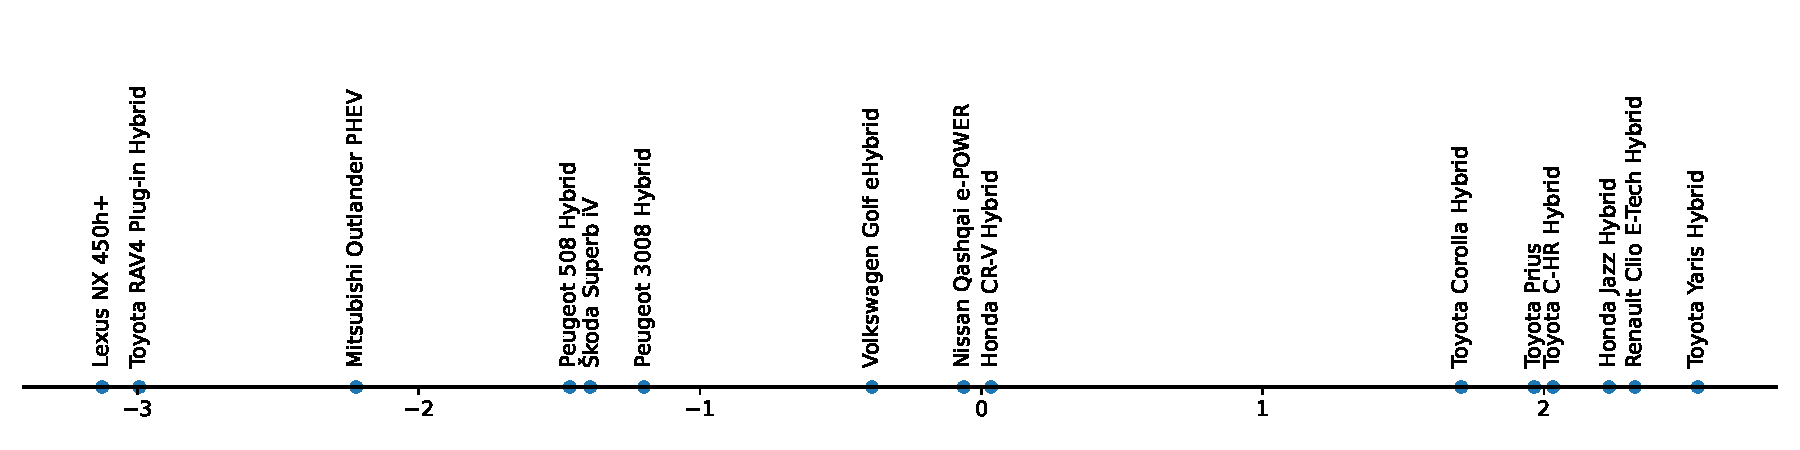
\includegraphics[width=\linewidth]{figs/050-cars.pdf}
    \caption{Rangiranje avtomobilov z metodo glavne komponente.}
    \label{fig:cars-rank}
\end{figure*}

Avtomobili v našem majhnem podatkovnem naboru razpadejo na nekaj skupin. Na desni so manjši, bolj ekonomični avtomobili, na levi pa bolj napredni, večji in najbrž tudi precej dražji. Cena ni bila vključena v tabelo, dodatno interpretacijo rezultatov pa predajamo bralcu. A očitno je, da je tudi tako preprosta tehnika in vizualizacija njenih rezultatov koristna in nudi številne možnosti njene interpretacije. Seveda bi nas pri interpretaciji zanimalo tudi, kakšen je vpliv posameznih atributov, oziroma kakšne so njihove uteži (angl. {\em loadings}). Tu so:

\vspace*{3mm}
\begin{lstlisting}
-0.501: Horsepower
-0.476: kWh/100 km
 0.454: 0-100 km/h (s)
-0.449: Type
-0.339: Trunk Size (L)
\end{lstlisting}

Največji vpliv ima moč motorja (\texttt{horsepower}), tesno ji sledi poraba električne energije (\texttt{kWh/100 km}), nato pa še pospešek, tip pogona in velikost prtljažnika. Negativni predznaki pri moči, porabi in tipu nakazujejo, da večji, zmogljivejši in praviloma priključni hibridi ležijo na enem koncu osi, medtem ko pozitivni prispevek časa pospeška pomeni, da počasnejši, manj zmogljivi avtomobili ležijo na drugem. Glavna komponenta tako v veliki meri pojasni prehod od manjših, manj zmogljivih in varčnejših vozil k večjim, zmogljivejšim in energijsko zahtevnejšim.

\section{Varianca v večrazsežnih prostorih}

Doslej smo razpršenost podatkov merili v eni dimenziji, kjer je varianca določena kot povprečje kvadratov odklonov od centra podatkov. Kako pa merimo razpršenost, kadar so podatki večrazsežni? Naj bodo podatki $x_1, \dots, x_n \in \mathbb{R}^d$. Predpostavimo, da so centrirani, torej $\bar{x} = 0$. Naravna posplošitev variance v večrazsežnem prostoru je
\[
\mathrm{Var}(X) = \frac{1}{n} \sum_{i=1}^n \|x_i\|^2,
\]
kjer $\|x_i\|$ označuje evklidsko normo vektorja $x_i$. Ta definicija ima smisel le, če predpostavimo, da je prostor $\mathbb{R}^d$ evklidski, torej opremljen z evklidsko geometrijo in z običajnim skalarnim produktom
\[
x^\top y = \sum_{j=1}^d x_j y_j,
\]
in pripadajočo normo $\|x\|^2 = x^\top x$. V takem prostoru veljajo znani geometrijski zakoni, med drugim Pitagorov izrek.

\medskip

\textbf{Trditev.} Če so podatki zapisani po koordinatah $x_i = (x_{i1}, \dots, x_{id})$, potem velja
\[
\mathrm{Var}(X) = \sum_{j=1}^d \mathrm{Var}(X^{(j)}),
\]
kjer $X^{(j)}$ označuje $j$-to koordinato podatkov.

\medskip

\textbf{Dokaz.} Začnimo z definicijo večrazsežne variance:
\[
\mathrm{Var}(X) = \frac{1}{n} \sum_{i=1}^n \|x_i\|^2.
\]
Ker uporabljamo evklidsko normo, lahko kvadrat norme razpišemo po koordinatah:
\[
\|x_i\|^2 = \sum_{j=1}^d x_{ij}^2.
\]
Vstavimo:
\[
\mathrm{Var}(X) = \frac{1}{n} \sum_{i=1}^n \sum_{j=1}^d x_{ij}^2.
\]
Zamenjamo vrstni red seštevanja:
\[
\mathrm{Var}(X) = \sum_{j=1}^d \left( \frac{1}{n} \sum_{i=1}^n x_{ij}^2 \right).
\]
Izraz v oklepaju pa je natanko varianca $j$-te koordinate:
\[
\mathrm{Var}(X^{(j)}) = \frac{1}{n} \sum_{i=1}^n x_{ij}^2.
\]
S tem dobimo
\[
\mathrm{Var}(X) = \sum_{j=1}^d \mathrm{Var}(X^{(j)}).
\]
\hfill $\square$

\medskip

Rezultat pove, da se v evklidskem prostoru skupna razpršenost podatkov razstavi na prispevke posameznih koordinat. To je neposredna posledica Pitagorovega izreka: kvadrat dolžine vektorja je vsota kvadratov njegovih projekcij na ortogonalne osi.

Ker se variance
%
\marginnote{Delež razložene variance (angl.~\emph{explained variance}) pove, kolikšen del celotne variance podatkov zajamemo z izbrano projekcijo. Če je skupna varianca podatkov $\mathrm{Var}(X)$, varianca projekcije na smer $u$ pa $\mathrm{Var}(Xu)$, potem je delež razložene variance enak $\mathrm{Var}(Xu) / \mathrm{Var}(X)$. Ta količina meri, koliko informacije (v smislu razpršenosti) ohranimo po projekciji.}
%
seštevajo po oseh, in ker so bili podatki na sliki~\ref{fig:data} standardizirani, lahko zaključimo, da je skupna varianca obeh teh podatkovnih naborov enaka 2. Projekcije na smer $a$ s slike~\ref{fig:ab} potem razložijo $1,902/2,0=95\%$ variance v podatkih, te na smer $b$ pa samo $1,541/2,0=77\%$. Z {\em razložijo} smo mislili, kolikšen delež celotne razpršenosti podatkov zajamemo, če podatke predstavimo le z njihovo projekcijo na izbrano smer. 

\section{Analiza glavnih komponent}

Zgornja lastnost, to je, da lahko v evklidskem prostoru skupno varianco razstavimo na vsoto varianc po posameznih koordinatnih oseh, je ključna tudi za razumevanje analize glavnih komponent. Cilj je poiskati nov koordinatni sistem, kjer so osi med seboj ortogonalne, in kjer se bo skupna varianca ponovno razdelila na vsoto varianc po teh novih oseh. Metoda glavnih komponent je tehnika, kjer izbere tak koordinatni sistem, kjer je večina variance zbrana v čim manjšem številu osi, tako da prva os zajame največji možni delež variance, druga os največji možni delež preostale variance, in tako naprej.

Analizo glavnih komponent 
%
\marginnote{Analizo glavnih komponent (PCA) je uvedel Karl Pearson leta 1901 kot nadaljevanje svojega dela na področju korelacij in kovariančne strukture podatkov, kjer je iskal načine za opis večrazsežnih podatkov z manjšim številom spremenljivk. Harold Hotelling pa je metodo v 1930-ih sistematiziral, uvedel njeno ime ter jo formalno povezal z lastnim razcepom kovariančne matrike in zaporednim iskanjem ortogonalnih komponent.}
%
(angl. PCA, {\em principal component analysis}) mnogokrat uporabimo za iskanje dvodimenzionalne projekcije, saj lahko podatke nato prikažemo v razsevnem diagramu. Naš razred \texttt{PCA1D} lahko razširimo v razred \texttt{PCA2D}, kjer istočasno iščemo dva smerna vektorja $u_1$ in $u_2$, ki sta enotska, med seboj pravokotna, in določata smeri največje skupne variance projekcij. Pri tem mora postopek zagotoviti, da $u_1$ zajame največjo varianco, $u_2$ pa največjo varianco med vsemi smermi, ki so ortogonalne na $u_1$.

Pri tem velja opozoriti, da optimizacija vsote varianc po dveh ortogonalnih smereh določi dvodimenzionalni podprostor največje razložene variance. Posamezni komponenti znotraj tega podprostora pa nista nujno enolično določeni, razen če dodatno zahtevamo, da je prva smer tista z največjo varianco, druga pa pravokotna nanjo in med takimi najbolj variabilna.

Da ohranimo ortogonalnost med vektorjema med optimizacijo, uporabimo Gram--Schmidtovo ortogonalizacijo. Najprej predpostavimo, da imamo dva vektorja $v_1$ in $v_2$, ki ju želimo pretvoriti v ortonormiran par $u_1, u_2$. Postopek poteka v dveh korakih, in sicer z normalizacijo prvega vektorja:
\[
u_1 = \frac{v_1}{\|v_1\|}.
\]
%
in odštevanje projekcije in normalizacija drugega vektorja, kjer najprej iz $v_2$ odstranimo komponento v smeri $u_1$,
\[
\tilde{v}_2 = v_2 - (v_2^\top u_1)\, u_1,
\]
% nato pa dobljeni vektor normiramo:
\[
u_2 = \frac{\tilde{v}_2}{\|\tilde{v}_2\|}.
\]
%
S tem zagotovimo, da velja $u_1^\top u_2 = 0$ in $\|u_1\| = \|u_2\| = 1$. Intuitivno drugi vektor ``očistimo'' komponente v smeri prvega, kar je neposredna posledica Pitagorovega izreka: preostanek leži v pravokotni smeri.


Naša implementacija sledi tej, ki smo jo uporabili za razred \texttt{PCA1D}:
\vspace*{3mm}
\begin{lstlisting}
class PCA2D:
    def __init__(self, n_inputs, rnd_seed=42):
        rng = random.Random(rnd_seed)
        self.v1 = [Value(rng.uniform(-1, 1), label=f"v1_{i}") for i in range(n_inputs)]
        self.v2 = [Value(rng.uniform(-1, 1), label=f"v2_{i}") for i in range(n_inputs)]

    def parameters(self):
        return self.v1 + self.v2

    def _dot(self, a, b):
        return sum(ai * bi for ai, bi in zip(a, b))

    def _norm(self, v, eps=1e-8):
        return (self._dot(v, v) + eps) ** 0.5

    def orthonormal_basis(self):
        # Gram-Schmidt orthonormalization
        nrm1 = self._norm(self.v1)
        u1 = [vi / nrm1 for vi in self.v1]

        proj_v2_on_u1 = self._dot(self.v2, u1)
        v2_orth = [v2i - proj_v2_on_u1 * u1i for v2i, u1i in zip(self.v2, u1)]
        nrm2 = self._norm(v2_orth)
        u2 = [v / nrm2 for v in v2_orth]
        return u1, u2

    def loss(self, xs, ys=None):
        # Maximize projected variance on two orthonormal axes.
        u1, u2 = self.orthonormal_basis()
        total = Value(0.0, label="proj_var_sum_2d")
        for x in xs:
            z1 = self._dot(x, u1)
            z2 = self._dot(x, u2)
            total += z1**2 + z2**2
        explained_var = total / len(xs)
        return -explained_var

    def batch_loss(self, xs, ys=None, m=20):
        indices = random.sample(range(len(xs)), m)
        batch_xs = [xs[idx] for idx in indices]
        return self.loss(batch_xs, ys=None)
\end{lstlisting}

V primerjavi z razredom \texttt{PCA1D} je ključna razlika ta, da tukaj optimiziramo dva smerna vektorja hkrati. Namesto enega vektorja $u$ imamo dva kandidata $v_1$ in $v_2$, ki ju med vsakim izračunom pretvorimo v ortonormirano bazo $(u_1, u_2)$ z Gram--Schmidtovim postopkom. Funkcija izgube tako ne meri več variance projekcije na eno smer, temveč vsoto varianc projekcij na obe smeri. S tem zajamemo skupno razpršenost podatkov v dvodimenzionalni podprostor. Pomembno je tudi, da ortogonalizacijo izvajamo sproti (znotraj metode \texttt{orthonormal\_basis}), zato ni treba eksplicitno omejevati parametrov — pogoj pravokotnosti in enotske dolžine je zagotovljen konstrukcijsko. Tako razširjena metoda dejansko išče prvi dve glavni komponenti hkrati.

Program tudi tu konvergira hitro. V namene analize izpišemo deleže razložene variance
%
\vspace*{3mm}
\begin{lstlisting}
Total variance: 5.000
Explained variance (PC1): 2.413 (48.3%)
Explained variance (PC2): 2.102 (42.0%)
Total explained variance (PC1+PC2): 4.515 (90.3%)
\end{lstlisting}
%
ter pojasnimo sestavo posameznih komponent,
\vspace*{3mm}
\begin{lstlisting}
Loadings, PC1:
 -0.630: Type
  0.444: 0-100 km/h (s)
 -0.392: Horsepower
 -0.370: kWh/100 km
  0.339: Trunk Size (L)

Loadings, PC2:
 -0.881: Trunk Size (L)
 -0.313: Horsepower
 -0.299: kWh/100 km
  0.187: 0-100 km/h (s)
  0.028: Type
\end{lstlisting}
% 
ter te uporabimo pri interpretaciji dobljene projekcije.

\begin{figure}
    \centering
    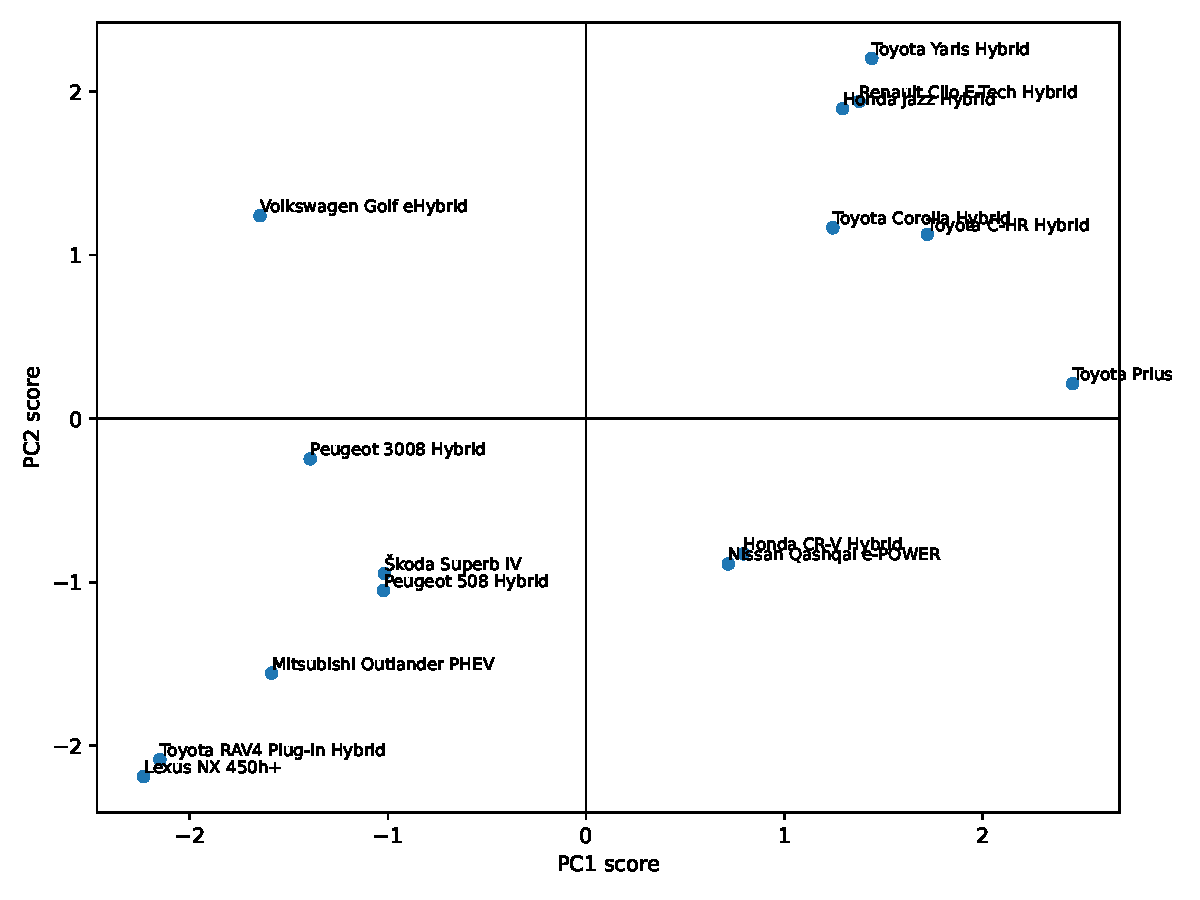
\includegraphics[width=\linewidth]{figs/050-cars-2d.pdf}
    \caption{Dvodimenzionalna projekcija podatkov o avtomobilih.}
    \label{fig:cars-2d}
\end{figure}

Prvi dve glavni komponenti torej zajameta več kot 90\% celotne variance. Dvodimenzionalna projekcija podatkov zato dobro ohranja strukturo podatkov. Prva komponenta (PC1) v največji meri ločuje vozila glede na zmogljivost in tip pogona, kar se kaže v večjih absolutnih utežeh pri atributih \texttt{Type}, \texttt{Horsepower} in \texttt{kWh/100 km}. Druga komponenta (PC2) pa je izrazito povezana z velikostjo vozila (predvsem \texttt{Trunk Size}), zato v vertikalni smeri razporeja avtomobile glede na prostornost. Na sliki~\ref{fig:cars-2d} tako jasno opazimo skupine vozil: manjši, varčnejši modeli se pojavljajo v zgornjem delu prostora, večji in zmogljivejši (pogosto priključni hibridi) pa v drugem, spodnjem, kar potrjuje, da PCA uspešno razkrije glavne vzorce v podatkih.

\section{Nekaj lastnosti v povezavi s korelacijami atributov}

Ponovimo na kratko: v evklidskem prostoru se variance po ortogonalnih oseh seštevajo. Če so atributi standardizirani, je varianca po vsaki osi enaka \(1\), zato je skupna varianca podatkov enaka številu atributov, \(d\). Prva glavna komponenta bo zato pojasnila več kot \(1/d\) celotne variance le tedaj, ko v podatkih obstaja neka struktura, to je, ko podatki niso zgolj naključno razmetani po prostoru.

To je intuitivno že v dveh dimenzijah. Pri podatkih s slike~\ref{fig:data} levo, kjer sta atributa nekorelirana in so podatki približno enakomerno razpršeni v vse smeri, lahko prvo komponento poljubno obračamo, pa bo vedno zajela približno polovico variance. Nobena smer namreč ni posebej izstopajoča. Za pojasnitev celotne variance zato nujno potrebujemo še drugo, pravokotno komponento. Podobno velja tudi v večrazsežnem prostoru: če so podatki približno sferično razporejeni, nobena komponenta ne bo izrazito pomembnejša od drugih.

PCA je zato najbolj uporabna takrat, ko med atributi obstajajo korelacije oziroma, širše, kadar podatki ležijo blizu nekega manjrazsežnega podprostora, recimo neke podravnine. V takem primeru glavne komponente kažejo v smeri največje razpršenosti podatkov, torej v smeri, kjer podatki nosijo največ informacije v smislu variance. Delež razložene variance po posamezni komponenti bo toliko večji od \(1/d\), kolikor izrazitejša je ta struktura.

Če želimo pojasniti prav vso varianco osnovnega prostora, moramo uporabiti vse glavne komponente. To pa navadno ni smiselno, saj s tem dimenzije sploh ne zmanjšamo. Namen PCA namreč ni modelirati prav vsega, tudi ne vsega šuma, ki je prisoten v podatkih. Pogosto nas zanima kompromis: obdržati le toliko komponent, da pojasnijo, denimo, \(80\%\) ali \(90\%\) celotne variance, preostanek pa zanemariti.

Pri tem velja nekaj previdnosti. Smeri z majhno varianco pogosto res ustrezajo šumu, vendar ne nujno vedno; v posameznih problemih lahko tudi te vsebujejo pomembno informacijo. PCA je zato predvsem uporabna metoda za stiskanje podatkov, vizualizacijo in odkrivanje strukture, ne pa nujno avtomatičen kriterij za ločevanje med signalom in šumom.

Pomembna lastnost PCA je tudi ta, da so glavne komponente med seboj ortogonalne, projekcije podatkov nanje pa nekorelirane. S tem dobimo nov koordinatni sistem, v katerem so informacije po posameznih oseh ločene oziroma nepodvojene.

S tem pridemo do glavnih uporab PCA: (1) vizualizacija podatkov v eni ali dveh dimenzijah, (2) zmanjšanje dimenzionalnosti in pogosto tudi delno odstranjevanje šuma ter (3) prehod v nov, dekoreliran prostor atributov. Kakšna enostavna linearna tehnika za analizo podatkov in tako zelo široko uporabo! In sploh še nismo na koncu. :)

\section{Regularizacija}

Predvsem pri podatkih v visokorazsežnih prostorih nas bo motilo to, da so uteži atributov za vsako od glavnih komponent neničelne. Želeli bi si namreč, da lahko vsako od osi pojasnimo le z manjšim delom atributov. Rešitev: L1 regularizacija! To že poznamo, in ker imamo tudi pri odkrivanju glavnih komponent opravka s cenovno funkcijo, lahko tudi v to dodamo regularizacijo. Dodatek je preprost, izgubi, ki smo jo izrazili kot delež razložene variance (z negativnim predznakom) dodamo še vsoto kvadriranih (L2) ali absolutnih (L1) vrednosti parametrov. Tu je dodatek:

\vspace*{3mm}
\begin{lstlisting}
params = self.parameters()
if self.reg == "l1":
    loss += self.reg_strength * sum([abs(p) for p in params]) / len(params)
elif self.reg == "l2":
    loss += self.reg_strength * sum([p**2 for p in params]) / len(params)
return loss
\end{lstlisting}

Pri postavitvi modela moramo zdaj dodati regularizacijske parametre, na primer z
%
\vspace*{3mm}
\begin{lstlisting}
pca = PCA2D(n_inputs=X.shape[1], reg="l1", reg_strength=3)
\end{lstlisting}
%
vse ostalo pa ostane popolnoma enako. Seveda bo na ta način model, torej naši glavni osi in nastala projekcija, drugačen od neregulariziranega. Konkretno, pri zgornjih nastavitvah, bodo uteži atributov, kot kaže spodnji izpis,
%
\vspace*{3mm}
\begin{lstlisting}
Loadings for PC1:
 -0.541: Horsepower
 -0.533: Type
 -0.532: kWh/100 km
 -0.323: Trunk Size (L)
 -0.188: 0-100 km/h (s)

Loadings for PC2:
  0.865: 0-100 km/h (s)
 -0.502: Trunk Size (L)
  0.000: Type
  0.000: kWh/100 km
  0.000: Horsepower
\end{lstlisting}
%
projekcija podatkov pa nekoliko drugačna:

\begin{figure}
    \centering
    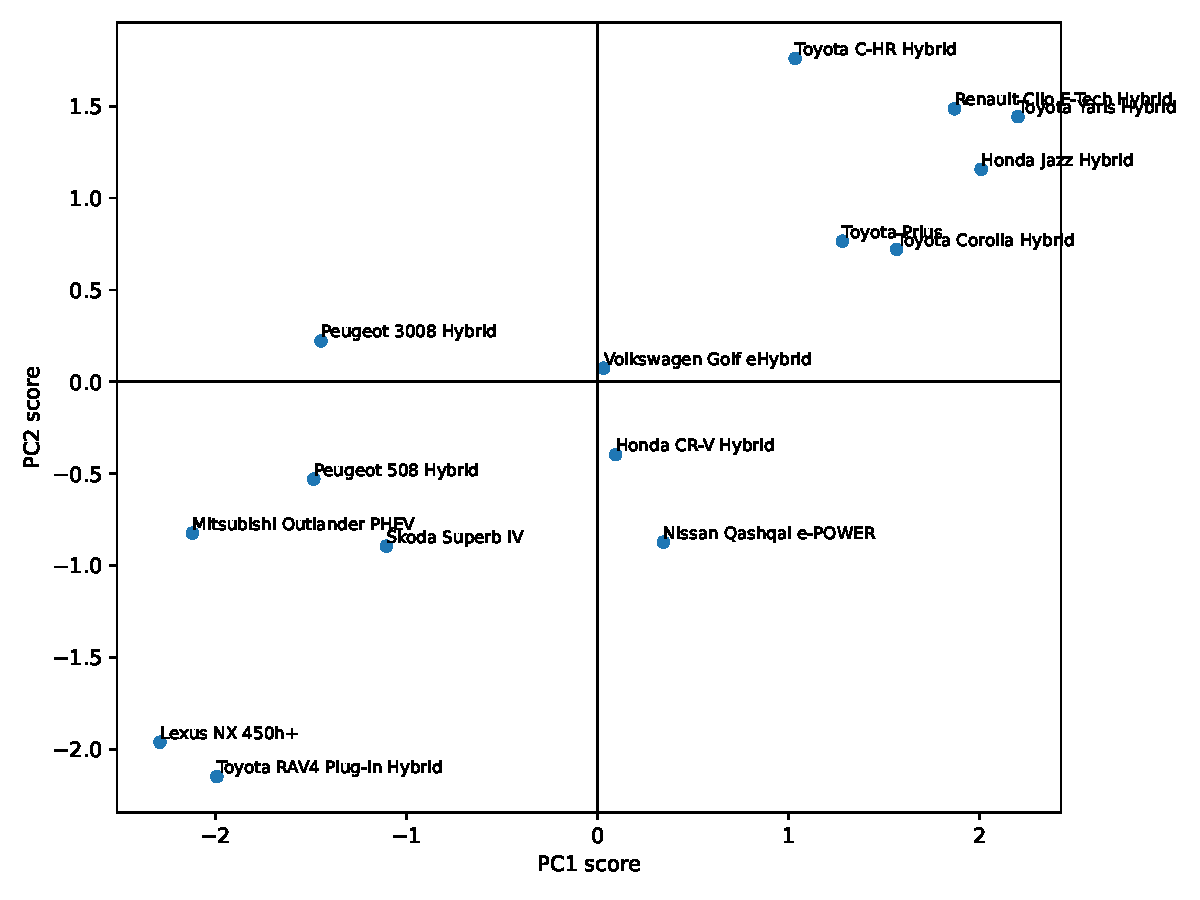
\includegraphics[width=\linewidth]{figs/050-cars-2d-reg.pdf}
    \caption{Dvodimenzionalna projekcija podatkov o avtomobilih, dobljena z regularizacijo L1 ($alpha=3$).}
    \label{fig:cars-2dr}
\end{figure}

Tu morda preseneča lahkota, s katero smo regularizacijo uvedli v metodo analize glavnih komponent. Klasična PCA sicer ima elegantno analitično rešitev\marginnote{PCA, klasično, temelji na lastnem razcepu kovariančne matrike $\Sigma = \tfrac{1}{n}X^\top X$: glavne komponente so lastni vektorji, pripadajoče lastne vrednosti pa podajajo razloženo varianco po posameznih smereh.}, a tak pristop je hkrati precej tog, saj je vezan na točno določeno kriterijsko funkcijo in ortogonalnost komponent. Ko želimo v model vključiti dodatne zahteve, na primer L1- ali L2-regularizacijo, analitična rešitev praviloma ni več na voljo in se moramo vrniti k numerični optimizaciji.

Analizo glavnih komponent lahko razumemo ne le kot zaprto matematično konstrukcijo, temveč tudi kot optimizacijski problem. S tem sicer izgubimo pot do klasične rešitve, a pridobimo tudi precej več svobode: kriterijski funkciji lahko dodajamo člene, ki spodbujajo gladkost, redkost ali druge želene lastnosti komponent. Gradientni sestop zato tu ni le didaktičen približek analitične rešitve, ampak splošnejši okvir, v katerem klasična PCA nastopa le kot njen najpreprostejši primer.

Zgoraj smo uporabili L1 regularizacijo kot primer načina izbora atributov, zmanjšanja kompleksnosti in pomoči pri lažji interpretaciji pomena komponent (uteži). Kako pa je lahko koristna regularizacija L2? Ne pozabimo: podatki, iz katerih gradimo nove, glavne komponente, so lahko šumni
%
\marginnote{Primer takih podatkov so lahko na primer meritve iz molekularne biologije, kjer nam sodobna tehnologija omogoča sočasno izmero več tisoč ali desettisoč spremenljivk (npr. genski izrazi), a bo zaradi cene in manjšega števila vzorcev (npr. merjenih tkiv) podatkov malo, možnost prevelike prilagoditve modela podatkom pa zato ogromna.}
%
. Tudi ta naš, sicer zelo enostaven model, se lahko preveč prilagodi šumu. Regularizacija L2 lahko to prilagoditev ublaži in razvije model, ki je bolj robusten. Za razliko od L1 regularizacije, ki spodbuja redkost in vodi do ničelnih uteži, L2 regularizacija uteži ne izniči, temveč jih enakomerno zmanjša. S tem prepreči, da bi posamezni atributi preveč dominirali pri določanju smeri glavnih komponent. Posledično dobimo bolj stabilne komponente, ki so manj občutljive na majhne spremembe v podatkih.

Intuitivno lahko rečemo, da L2 regularizacija nekoliko ``zgladi'' prostor rešitev: namesto da bi model izbral smer z maksimalno možno varianco, ki je lahko deloma posledica šuma, raje izbere bolj uravnoteženo smer, ki bolje odraža splošno strukturo podatkov. V tem smislu L2 regularizacija uvaja kompromis med maksimalno razloženo varianco in robustnostjo modela.


\section{Točnost, metaparametri učenja}

Zgoraj smo tudi v analizi glavnih komponent uvedli regularizacijo in s tem metaparameter stopnje regularizacije, parameter, katerega vrednost moramo oceniti. A kako? PCA ne napoveduje, kako lahko potem ocenimo kakovost modela in na tej osnovi izberemo primerno stopnjo regularizacije?

O ocenjevanju točnosti in izboru metaparametrov smo pisali že na koncu prejšnjega poglavja. Kvaliteto modela moramo vedno oceniti na ločeni, testni množici. Kvaliteta pri PCA ni vezana na napovedovanje, a smo tudi pri razvoju PCA določili kriterijsko funkcijo — stopnjo razložene variance — ki nam lahko služi za oceno, kako dober je naš model.

Postopek je zato močno podoben, ali bolj rečeno, v osnovni enak kot pri linearni regresiji: podatke razdelimo na učno in testno množico. Na učni množici zgradimo model (določimo glavne komponente), nato pa testne podatke projiciramo na te komponente in na tej projekciji izračunamo razloženo varianco. S tem ocenimo, kako dobro naučene komponente zajamejo strukturo novih podatkov. Pri tem moramo biti pozorni, da vse korake, kot je standardizacija podatkov, izvedemo na učni množici in nato enake transformacije uporabimo na testni množici. V nasprotnem primeru bi lahko nehote uporabili informacijo iz testnih podatkov. Pri tem razloženo varianco na testni množici vedno računamo glede na standardizacijo, naučeno na učni množici, saj bi sicer v oceno nehote vključili informacijo iz testnih podatkov.

Za ocenjevanje primerne vrednosti stopnje regularizacije lahko uporabimo isti trik kot pri linearni regresiji: celotno metodo (standardizacijo, izbor stopnje regularizacije na validacijski množici in gradnjo končnega modela s tako ocenjeno stopnjo regularizacije) zapremo v škatlo, in to v namene neodvisne ocene uspešnosti validiramo na testni množici. Za bolj robustno validacijo lahko tudi tu uporabimo prečno preverjanje. In za končni model celotno škatlo z našo metodo poženemo na vseh podatkih.

\section{Dodatek: glavne komponente so lastni vektorji kovariančne matrike}

V tem razdelku smo se metode PCA lotili z optimizacijo kriterijske funkcije, torej na nekonvencionalen način, tudi zato, ker se bomo s številnimi drugimi tehnikami, kjer nas bo zanimalo modeliranje in razlaga podatkov, spoprijeli prav na ta način. A ima PCA tudi lepo matematično in statistično izpeljavo in podlago in najbrž ne bi bilo prav, če je vsaj ne omenimo. Poteka po naslednjih korakih.

\begin{enumerate} 

\item {\bf Osrediščenje podatkov} Naj bodo \( X \) podatki dimenzij \( n \times d \), kjer je \( n \) število primerov in \( d \) število značilk. Privzamemo, da so podatki osrediščeni, kar pomeni, da za vsako značilko velja:
\[
\frac{1}{n} \sum_{i=1}^{n} X_{i,j} = 0, \quad \text{za vsak } j = 1, 2, \dots, d
\]

\item {\bf Iskanje prve komponente \( \mathbf{u}_1 \)}. Iščemo vektor \( \mathbf{u}_1 \) (dimenzije \( d \times 1 \)), ki določa prvo glavno komponento — smer v prostoru značilk, na katero, če projiciramo podatke, bo varianca projekcij največja. Projekcija podatkovne matrike \( X \) na \( \mathbf{u}_1 \) je:
\[
z = X \mathbf{u}_1
\]
Varianca projekcije \( z \) je:
\[
\mathrm{Var}(z) = \frac{1}{n} \| X \mathbf{u}_1 \|^2 = \frac{1}{n} \mathbf{u}_1^T X^T X \mathbf{u}_1
\]
Ker želimo poiskati smer $\mathbf{u}_1$ z maksimalno varianco, je naša kriterijska funkcija:
\[
\max_{\mathbf{u}_1} \mathbf{u}_1^T S \mathbf{u}_1
\]
kjer malce podrobnejši pogled na zgornjo strukturo pokaže, da je \( S = \frac{1}{n} X^T X \) kovariančna matrika podatkov. Pri tem omejimo dolžino vektorja \( \mathbf{u}_1 \) na 1. To je tudi pogoj, ki mu mora zadostiti kriterijska funkcija:
\[
\mathbf{u}_1^T \mathbf{u}_1 = 1
\]

\item {\bf Optimizacija.} Rešitev problema poiščemo z uporabo Lagrangeovih multiplikatorjev. Postavimo Lagrangeovo funkcijo:
\[
L(\mathbf{u}_1, \lambda) = \mathbf{u}_1^T S \mathbf{u}_1 - \lambda (\mathbf{u}_1^T \mathbf{u}_1 - 1)
\]
in poiščemo stacionarne točke:
\[
\frac{\partial L}{\partial \mathbf{u}_1} = 2 S \mathbf{u}_1 - 2 \lambda \mathbf{u}_1 = 0
\]
\[
S \mathbf{u}_1 = \lambda \mathbf{u}_1
\]
Zgornja enačba je lastna enačba kovariančne matrike. Torej je \( \mathbf{u}_1 \) lastni vektor kovariančne matrike \( S \), pripadajoča lastna vrednost \( \lambda \) pa je:
\[
S \mathbf{u}_1 = \lambda_1 \mathbf{u}_1
\]

\item {\bf Rešitev}. Varianca projekcije je torej podana z:
\[
\mathrm{Var}(z) = \frac{1}{n} \| X \mathbf{u}_1 \|^2 = \mathbf{u}_1^T S \mathbf{u}_1
\]
Ker pa iz lastne enačbe velja:
\[
S \mathbf{u}_1 = \lambda_1 \mathbf{u}_1
\]
sledi:
\[
\mathbf{u}_1^T S \mathbf{u}_1 = \mathbf{u}_1^T \lambda_1 \mathbf{u}_1 = \lambda_1 (\mathbf{u}_1^T \mathbf{u}_1) = \lambda_1
\]
ker smo predpostavili, da je \( \mathbf{u}_1^T \mathbf{u}_1 = 1 \). Zato velja:
\[
\mathrm{Var}(z) = \lambda_1
\]
kar pomeni, da je lastna vrednost \( \lambda_1 \) enaka varianci podatkov v smeri prve glavne komponente \( \mathbf{u}_1 \).

Ker želimo maksimizirati varianco projekcije, med vsemi možnimi lastnimi vektorji kovariančne matrike za prvo komponento vzamemo tisti lastni vektor, ki ustreza največji lastni vrednosti \( \lambda_1 \). Varianca v smeri \( \mathbf{u}_1 \) je enaka tej lastni vrednosti:
%
\[
\mathrm{Var}(z) = \lambda_1
\]
Vse ostale komponente so torej lastni vektorji, urejeni po padajočih lastnih vrednostih, ki podajajo razloženo varianco po posameznih komponentah.
\end{enumerate}

Zgornja izpeljava je elegantna in vzpostavi povezavo med glavnimi komponentami in prostorom lastnih vektorjev kovariančne matrike. Tu tudi postane jasno, zakaj so glavne komponente povezane s korelacijami med atributi. A kljub eleganci rešitve ta ne omogoča razširitev tehnike z regularizacijo, kjer je pristop, ki uporablja gradientni sestop, kot smo ga razvili v poglavju, prava rešitev.